\documentclass[]{article}


\usepackage{float} % inline figures

\usepackage{listings}
\usepackage{tikz}
\usetikzlibrary{arrows}


\def\codefont{
%	\fontspec{Courier New}
	\fontsize{9pt}{11pt}\selectfont}
\definecolor{codebgcolor}{HTML}{EDEDED}
\newenvironment{code}
{\begin{center}
		\begin{tikzpicture}
		\node [fill=codebgcolor,rounded corners=5pt]
		\bgroup
		\bgroup\codefont
		\begin{tabular}{l}}
	{\end{tabular}
		\egroup
		\egroup;
		\end{tikzpicture}
	\end{center}}


%\usepackage[pdftex]{graphicx} % allow images in subdirectory
%\graphicspath{{Figures/}}

\usepackage[margin=1in]{geometry} % reduce margins

\usepackage{url} % link URLs in document


%%% Paragraph numbering %%%
\usepackage{linguex}
% Counter format 
\renewcommand{\ExLBr}{\bfseries}
\renewcommand{\ExRBr}{}
% http://tex.stackexchange.com/a/57279/11604
% Reset \ex. at each section 
\usepackage{chngcntr}
\counterwithin{ExNo}{subsection}
% add section counter
\renewcommand{\Exarabic}{\thesubsection.\arabic} 
\AtBeginDocument{\setlength{\Exindent}{0pt}}

%%%%%%%%%%%%%%%%%%%%%%%%%%%%

%opening
\title{Synchronization of PNA Measurements with SMUs for DC Biasing.}
\author{Jackson Anderson}

\begin{document}


\maketitle


\section{Introduction}
This document serves as a guide for setup and execution of measurements using the Keysight N5225 parametric network analyzer as a remote GPIB controller. 


\section{Change Log}

v1.0, Nov. 22, 2017 : Document Created
\\ \\
v1.1, Apr. 25, 2018 : Added figure captions, cleaned up document.


\newpage
\section{Initial Setup for Windows}

\subsection{VISA Driver Installation}

\ex. Navigate to \url{https://www.keysight.com/}. In the upper right section of the screen, search for IO Libraries Suite. The product should appear at the top of the search results. Click on \textbf{product details} to navigate to the product page. In the center of the screen, select \textbf{Trials \& Licenses} in the center of the screen, followed by \textbf{Details \& Download}. This will bring you to the download page for the current version. Click \textbf{Download} and run the installer to install Keysight Connection Expert on your PC, which will be used to set up communication to a remote GPIB network over LAN using the PNA as the GPIB controller. 

\begin{figure}[H]
	\centering
	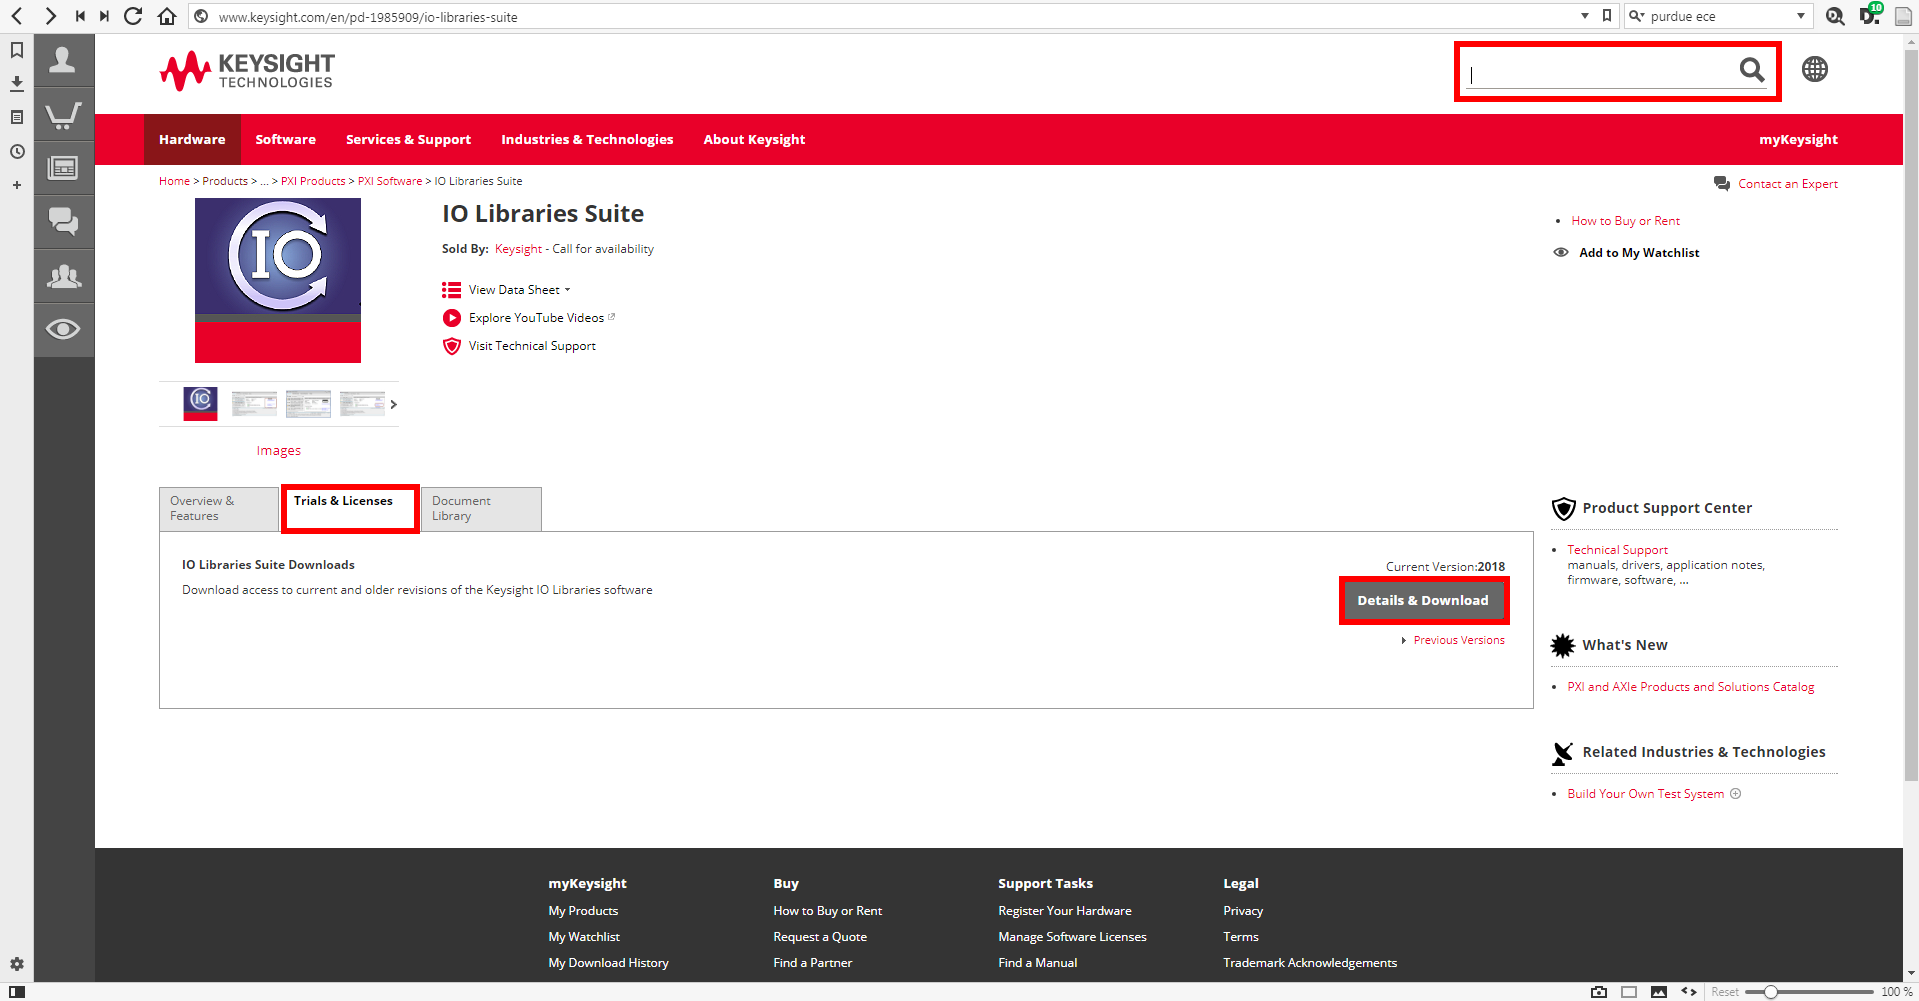
\includegraphics[width=\linewidth]{Figures/keysight}
	\caption{Keithley IO Libraries Suite webpage.}
	\label{fig:kcon}
\end{figure}


\ex. Navigate to \url{http://www.ni.com/downloads/}. Using the search bar on the left, select \textbf{Drivers} then \textbf{NI Drivers}. In the "Narrow by" section under products, select \textbf{Instrument Connectivity} $->$ \textbf{GPIB} $->$ \textbf{GPIB Software} $->$ \textbf{NI-VISA}. You should now see only NI-VISA downloads; download and install the latest version for your system.

\begin{figure}[H]
	\centering
	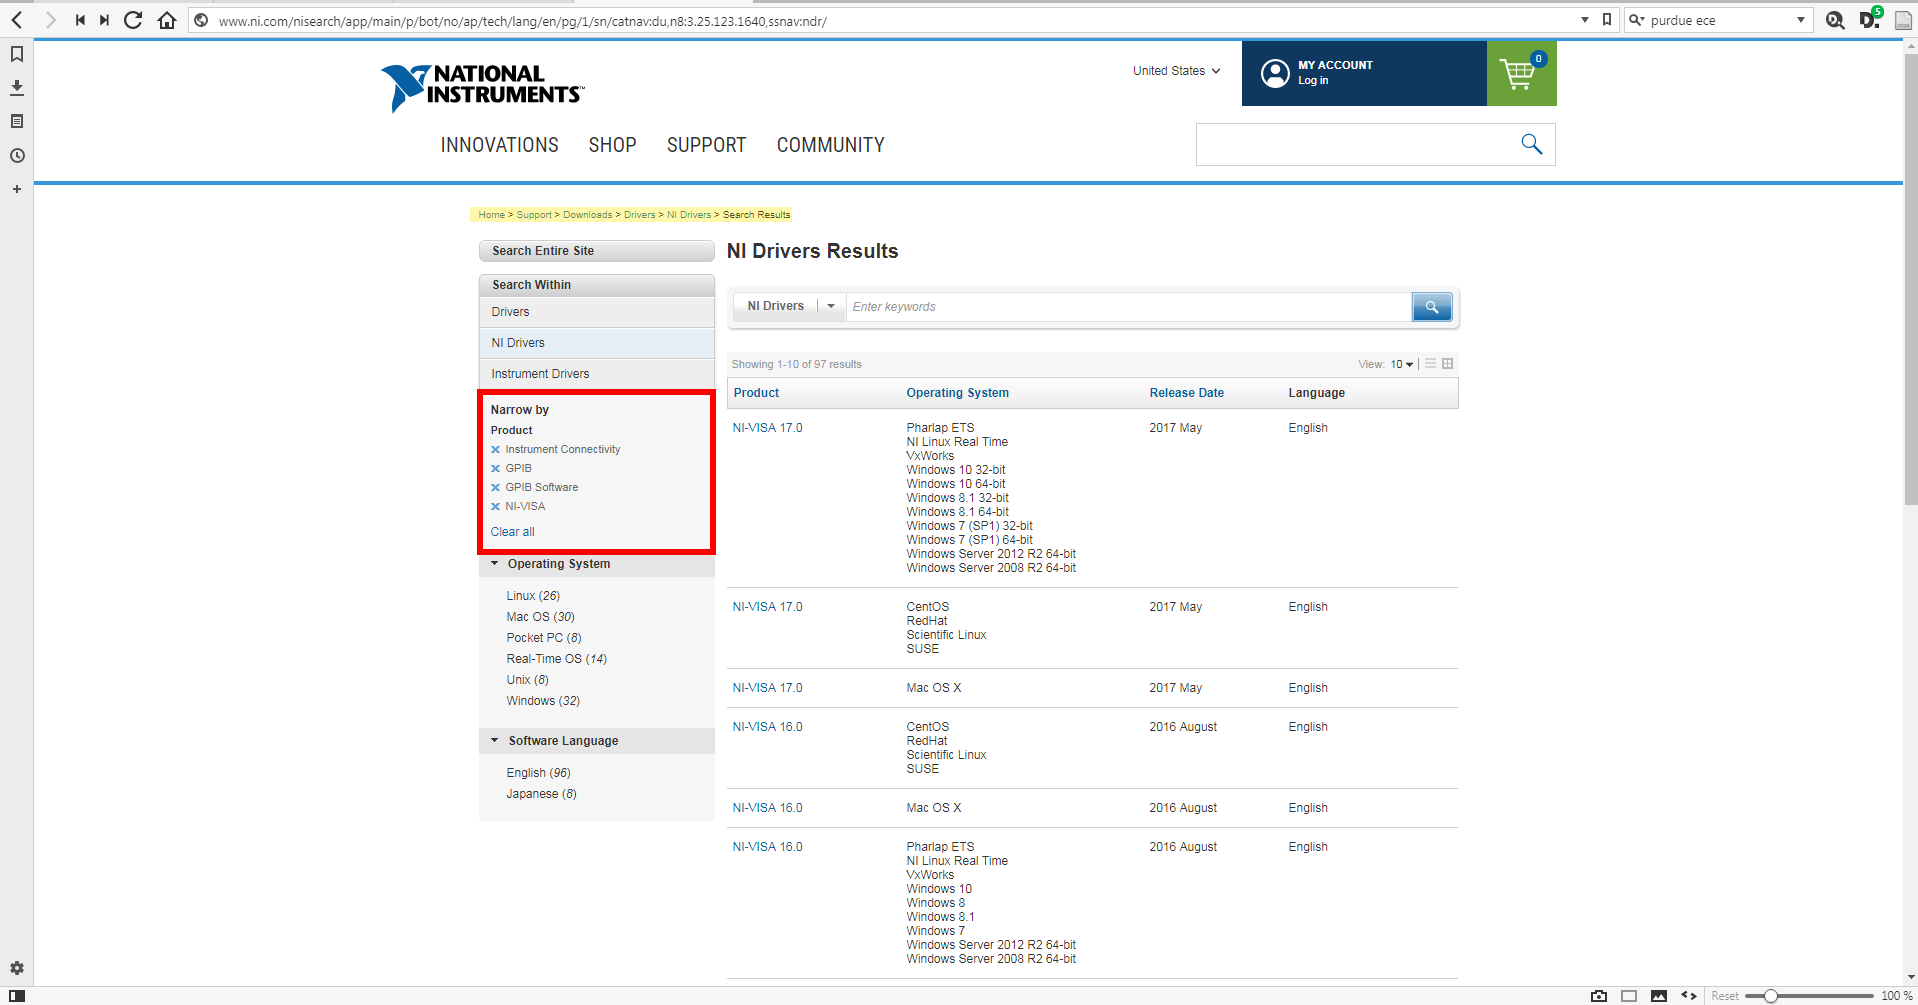
\includegraphics[width=\linewidth]{Figures/nivisa}
	\caption{NI VISA drivers download webpage. }
	\label{fig:nivisa}
\end{figure}



\subsection{GPIB Network Setup}

\ex. Connect your computer to the PNA with an ethernet cord. 

\ex. In order to communicate with the PNA, your computer's ethernet adapter settings must be set up to match those of the PNA. Open the \textbf{Network and Sharing Center} in the Control Panel and select \textbf{Change adapter settings} on the left side of the window.


\begin{figure}[H]
	\centering
	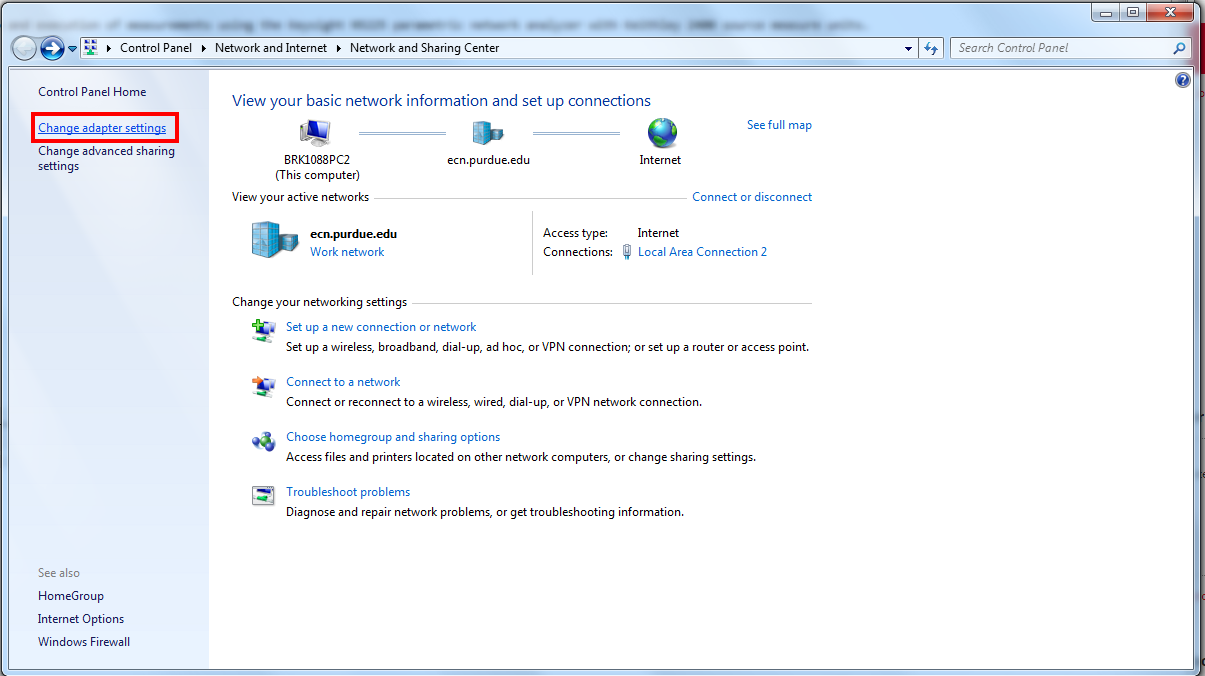
\includegraphics[width=\linewidth]{Figures/cp1}
	\caption{Windows Network and Sharing Center.}
	\label{fig:cp1}
\end{figure}

\ex. Right click on your ethernet adapter and select \textbf{Properties}. In \textbf{Ethernet Properties}, select \textbf{Internet Protocol Version 4 (TCP/IPv4)} and click \textbf{Properties}. 

\ex. In the window that appears, select "Use the following IP address." The PNA uses a default gateway of 192.168.1.2 and a subnet mask of 255.255.255.0. For IP address, enter a value 192.168.1.xx, where the last term is some number besides 1 (used by the PNA) and 2 (the default gateway). Once this is done, select OK and then OK to close out of the IPv4 and Ethernet Properties windows.

\begin{figure}[H]
	\centering
	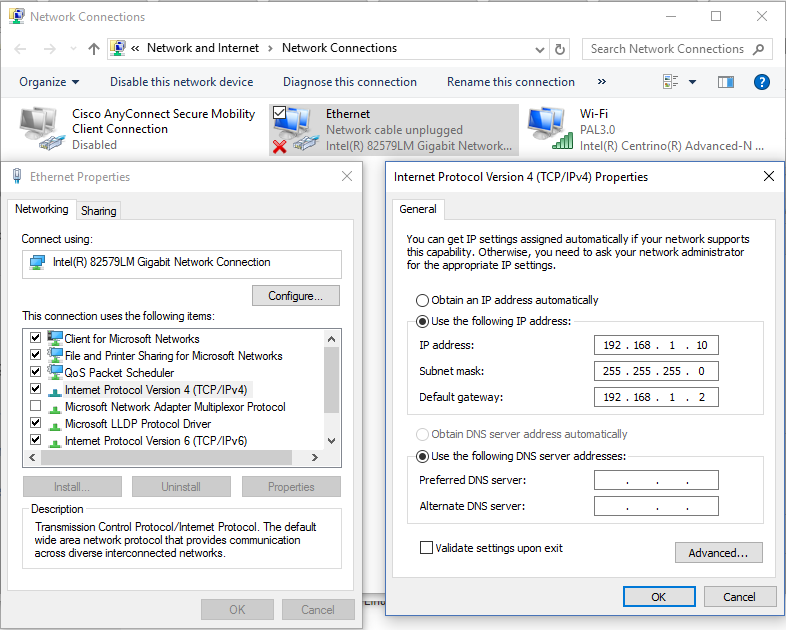
\includegraphics[width=\linewidth]{Figures/network}
	\caption{Adapter Settings menu for Windows 10. These settings can be customized as desired, as long as they match the PNA setup.}
	\label{fig:cp2}
\end{figure}

\ex. The final step before we can make measurements is to set up the remote GPIB network so that your PC can communicate to the SMUs as if it was the GPIB controller. This is done in Keysight Connection Expert. Open Keysight Connection Expert. If your ethernet is set up correctly, the PNA should be detected and appear on the \textbf{Instruments} tab. Select the \textbf{Manual Configuration} tab along the top of the screen. Under \textbf{Add New Instruments/Interfaces} on the left, select \textbf{Remote GPIB interface}. Ensure options match those shown in the figure below, then select \textbf{Test Connection} to verify the settings. If the test is successful, select \textbf{Accept}. You should now be able to control the PNA and SMUs remotely.

\begin{figure}[H]
	\centering
	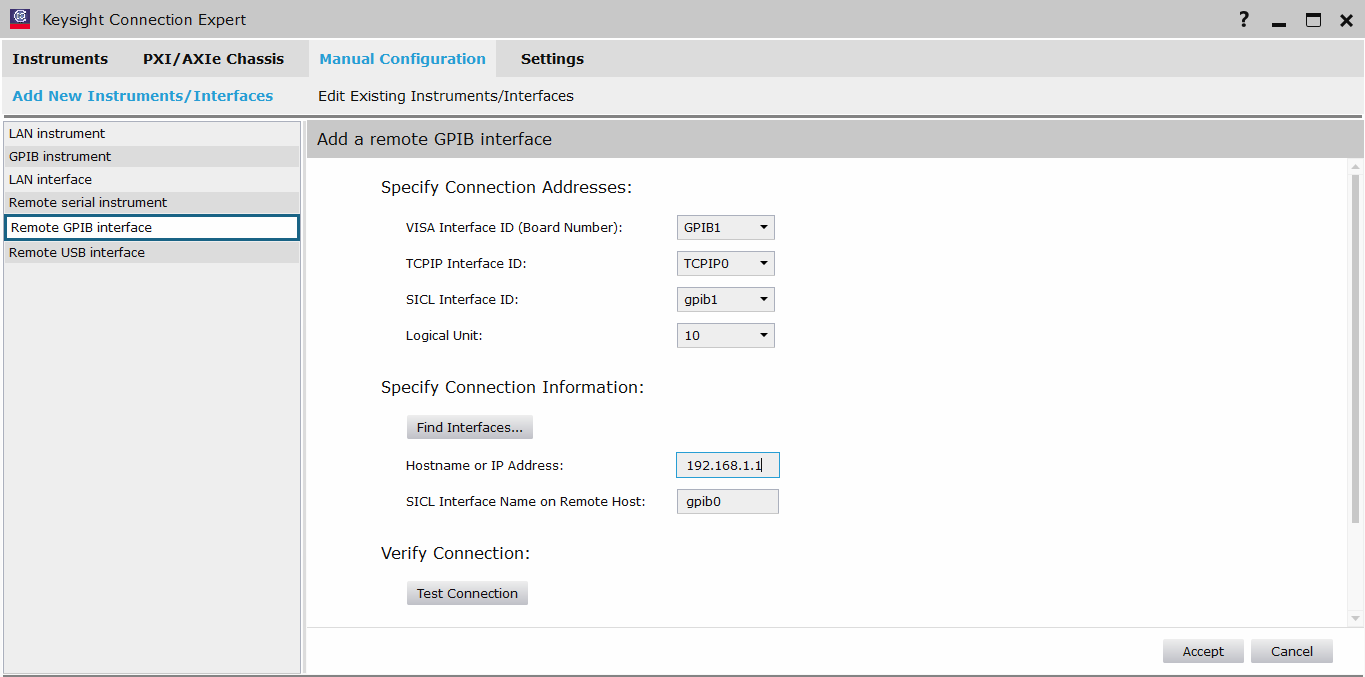
\includegraphics[width=\linewidth]{Figures/kce}
	\caption{Setting up the remote GPIB network in Keysight Connection Expert.}
	\label{fig:kce}
\end{figure}

\subsection{Python Setup}

\ex. In order to make measurements using the code in this repository, you will need Python 3 installed on your measurement control computer. Navigate to \url{https://www.anaconda.com/download/} and download the Python 3.6 version of Anaconda. Choose 32- or 64-bit based on your system. If you are on Windows and are not sure about your system bitness, right click on \textbf{My Computer} (\textbf{This PC} in Windows 10), click \textbf{Properties}, and the version should be listed under System Type.

\begin{figure}[H]
	\centering
	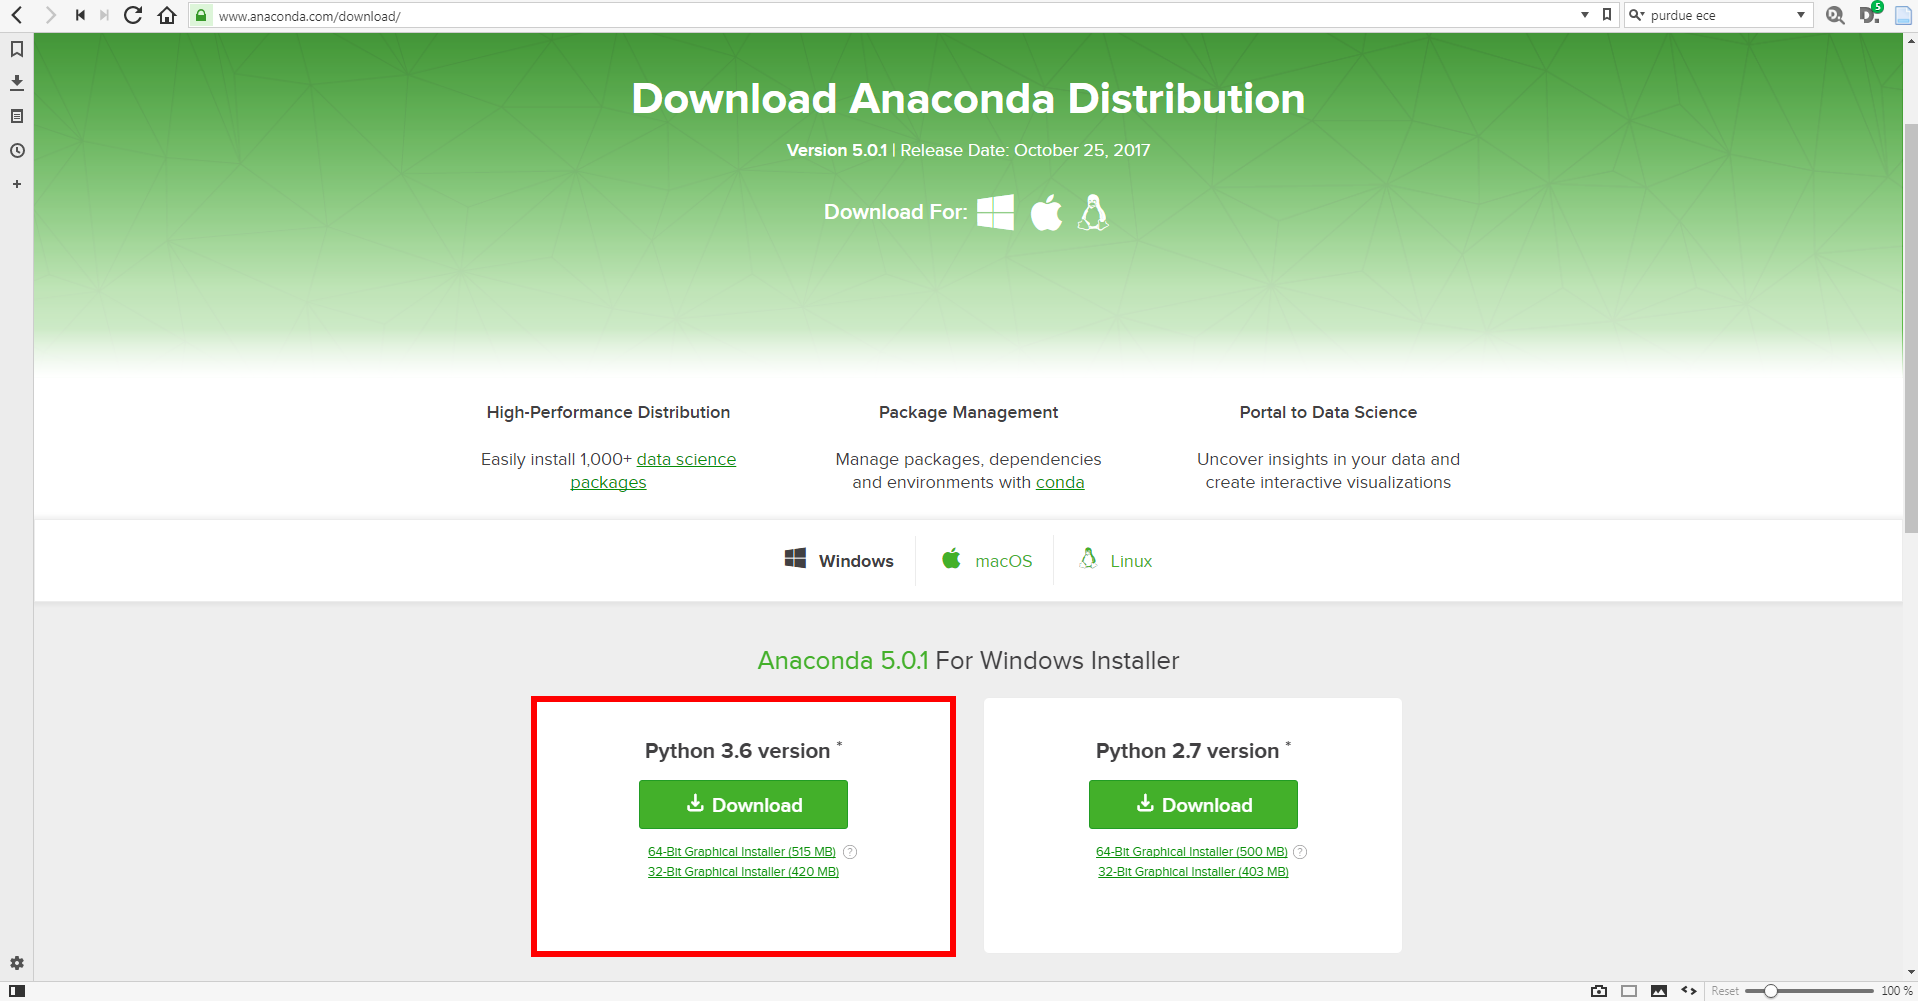
\includegraphics[width=\linewidth]{Figures/anaconda}
	\caption{Anaconda Python distribution webpage. Be sure to download Python version 3.x for use.}
	\label{fig:anaconda}
\end{figure}


\ex. Run the anaconda installer, agreeing to the default settings.

\ex. If downloading this code from GitHub for use, you must ensure that you have the prerequisite packages installed. Open the start menu, click on the anaconda folder that was created during installation, and open the anaconda prompt as an administrator (right click, select \textbf{Run as Administrator}).

\begin{figure}[H]
	\centering
	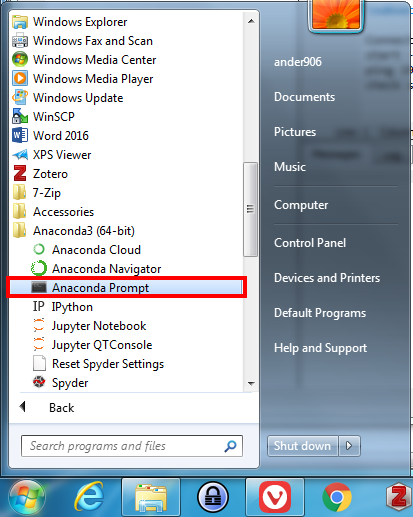
\includegraphics[width=0.4\linewidth]{Figures/py1}
	\caption{Opening the Anaconda prompt.}
	\label{fig:py1}
\end{figure}

\ex. Once the terminal window opens and the prompt appears, type the following and press enter:

\begin{code}
	\begin{lstlisting}[language=python]
	conda install pip
	\end{lstlisting}
\end{code}

\ex. After verifying that pip is installed with the above command, the next step is to install the pyvisa package that will be used to communicate with the test instruments. Type the following and press enter:

\begin{code}
	\begin{lstlisting}[language=python]
	pip install visa
	\end{lstlisting}
\end{code}

\ex. You should now be able to run the code contained in this repository without errors.

\end{document}
